%%%%%%%%%%%%%%%%%%%%%%%%%%%%%%%%%%%%%%%%%

%----------------------------------------------------------------------------------------
%	PACKAGES AND OTHER DOCUMENT CONFIGURATIONS
%----------------------------------------------------------------------------------------

\documentclass{article}

\input{C:/Code/TexStudio/templates/structure.tex} % Include the file specifying the document structure and custom commands

%----------------------------------------------------------------------------------------
%	ASSIGNMENT INFORMATION
%----------------------------------------------------------------------------------------

\title{Assignment \#2} % Title of the assignment

\author{Name:Cao Mingming\\ Student ID:2018311770\\ \texttt{cmm18@mails.tsinghua.edu.cn}} % Author name and email address

\date{Tsinghua University --- \today} % University, school and/or department name(s) and a date

%----------------------------------------------------------------------------------------

\begin{document}

\maketitle % Print the title

%----------------------------------------------------------------------------------------
%	INTRODUCTION
%----------------------------------------------------------------------------------------
\section{Question 1}
Derive ABCD matrix for a curved mirror, a thin lens and a thick lens is illustrated as figure \ref{fig1}.
\section*{Solution}
\subsection{Thin lens}
The sketch map of a thins is illustrated as in figure 
\begin{figure}[h]
	\centering
	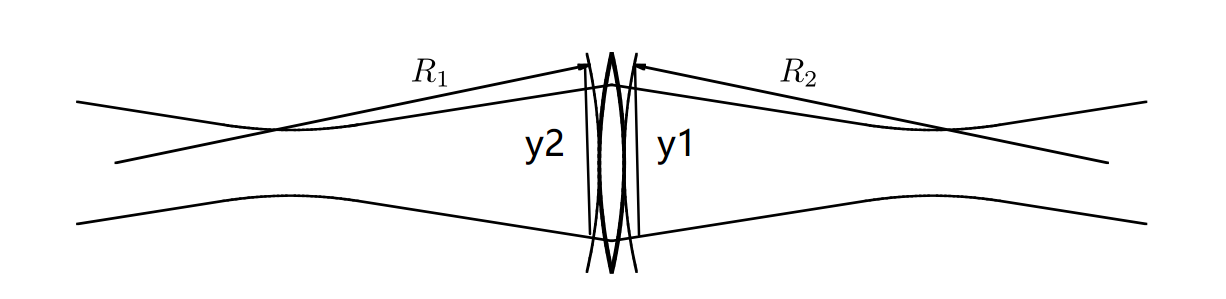
\includegraphics[width=8cm]{thin_lens.png}
	\caption{Thin lens}
	\label{fig1}
\end{figure}
Suppose that the spot size keeps unchange, by the simple lens formula we could get.
\begin{equation}\label{eq1}
\frac{1}{i}+\frac{1}{o}=\frac{1}{f}
\end{equation}
Take the image distance i as $ R_1 $, the object distance o is $ R_2 $ and f is the focal length.
\begin{equation}\label{eq2}
\frac{1}{R_1}-\frac{1}{R_2}=\frac{1}{f}
\end{equation}
Due to that the ray height is unchangd, and solpe can be obtained by len frmula
\begin{equation}\label{eq3}
y_1=y_2,\quad y_{2}^{'}=-\frac{y_2}{i},\quad y_{1}^{'}=\frac{y_1}{o}
\end{equation}
Substitute equation \ref{eq2} into equation \ref{eq3}, we can get
\begin{equation}\label{key}
\begin{array}{l}
y_2=y_1+0*y_{1}^{'}\\
\\
y_{2}^{'}=-\frac{y_1}{f}+y_{1}^{'}
\end{array}
\end{equation}
So the ABCD matrix of thin lens is,
\begin{equation}\label{eq5}
\left(
\begin{array}{cc}
1 & 0\\
-\frac{1}{f} & 0
\end{array}
\right)
\end{equation}

\subsection{Curved mirror}
Supposed that the radius of thin mirror is R, which menas that the focal length is $f=\frac{R}{2}$. Substitue f into equation \ref{eq5} we can get ABCD matrix of curved mirror is,
\begin{equation}\label{eq6}
\left(
\begin{array}{cc}
1 & 0\\
-\frac{2}{R} & 0
\end{array}
\right)
\end{equation}
And the z direction (propagation direction) gets inversed after mirror.
\subsection{Thick Lens}
As is shown in figure \ref{fig2} the radii of a thick lens are $ R_1 $ and $ R_2 $, thickness is $ d $ and the refractive index are $ n_1 $ and $ n_2 $.
\begin{figure}[h]
	\centering
	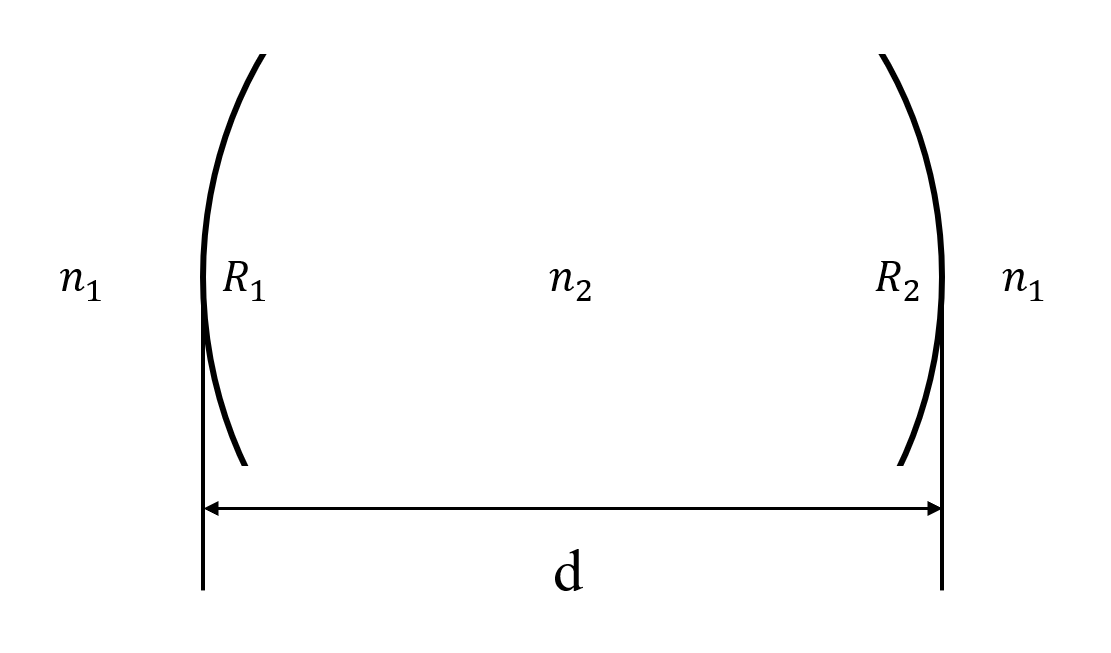
\includegraphics[width=8cm]{thick_lens.png}
	\caption{Thick lens}
	\label{fig3}
\end{figure}
It can be decomposed into three parts, a refraction part with radius of $ R_1 $, a propagation part with length d and a refraction part with radius of $ -R_2 $. Therefore the ABCD matrix can be written as,
\begin{equation}\label{eq7}
A=A_3*A_2*A_1
\end{equation}
where $ A_1,\quad A_2,\quad A_3 $ are the ABCD matrixes of the three part metntioned above. Substitute
$$
\begin{array}{l}
A_1=
\left(
\begin{array}{cc}
1 & 0\\
\frac{n_1-n_2}{n_2R_1} & \frac{n_1}{n_2}
\end{array}
\right)
\end{array}
$$

$$
\begin{array}{l}
A_2=
\left(
\begin{array}{cc}
1 & d\\
0 & 1
\end{array}
\right)
\end{array}
$$

$$
\begin{array}{l}
A_3=
\left(
\begin{array}{cc}
1 & 0\\
\frac{n_2-n_1}{n_1R_2} & \frac{n_2}{n_1}
\end{array}
\right)
\end{array}
$$
into equation \ref{eq7} we can derive that
\begin{equation}\label{key}
A=\left(
\begin{array}{cc}
1+\frac{d(n_1-n_2)}{R_1n_2} & d\frac{n_1}{n_2} \\
\\
\frac{(n_1-n_2)n_2(R_2-R_1)-d(n_1-n_2)^2}{n_1n_2R_1R_2}& 1+\frac{d(n_2-n_1)}{R_2n_2}
\end{array}
\right)
\end{equation}
\begin{figure}[h]
	\centering
	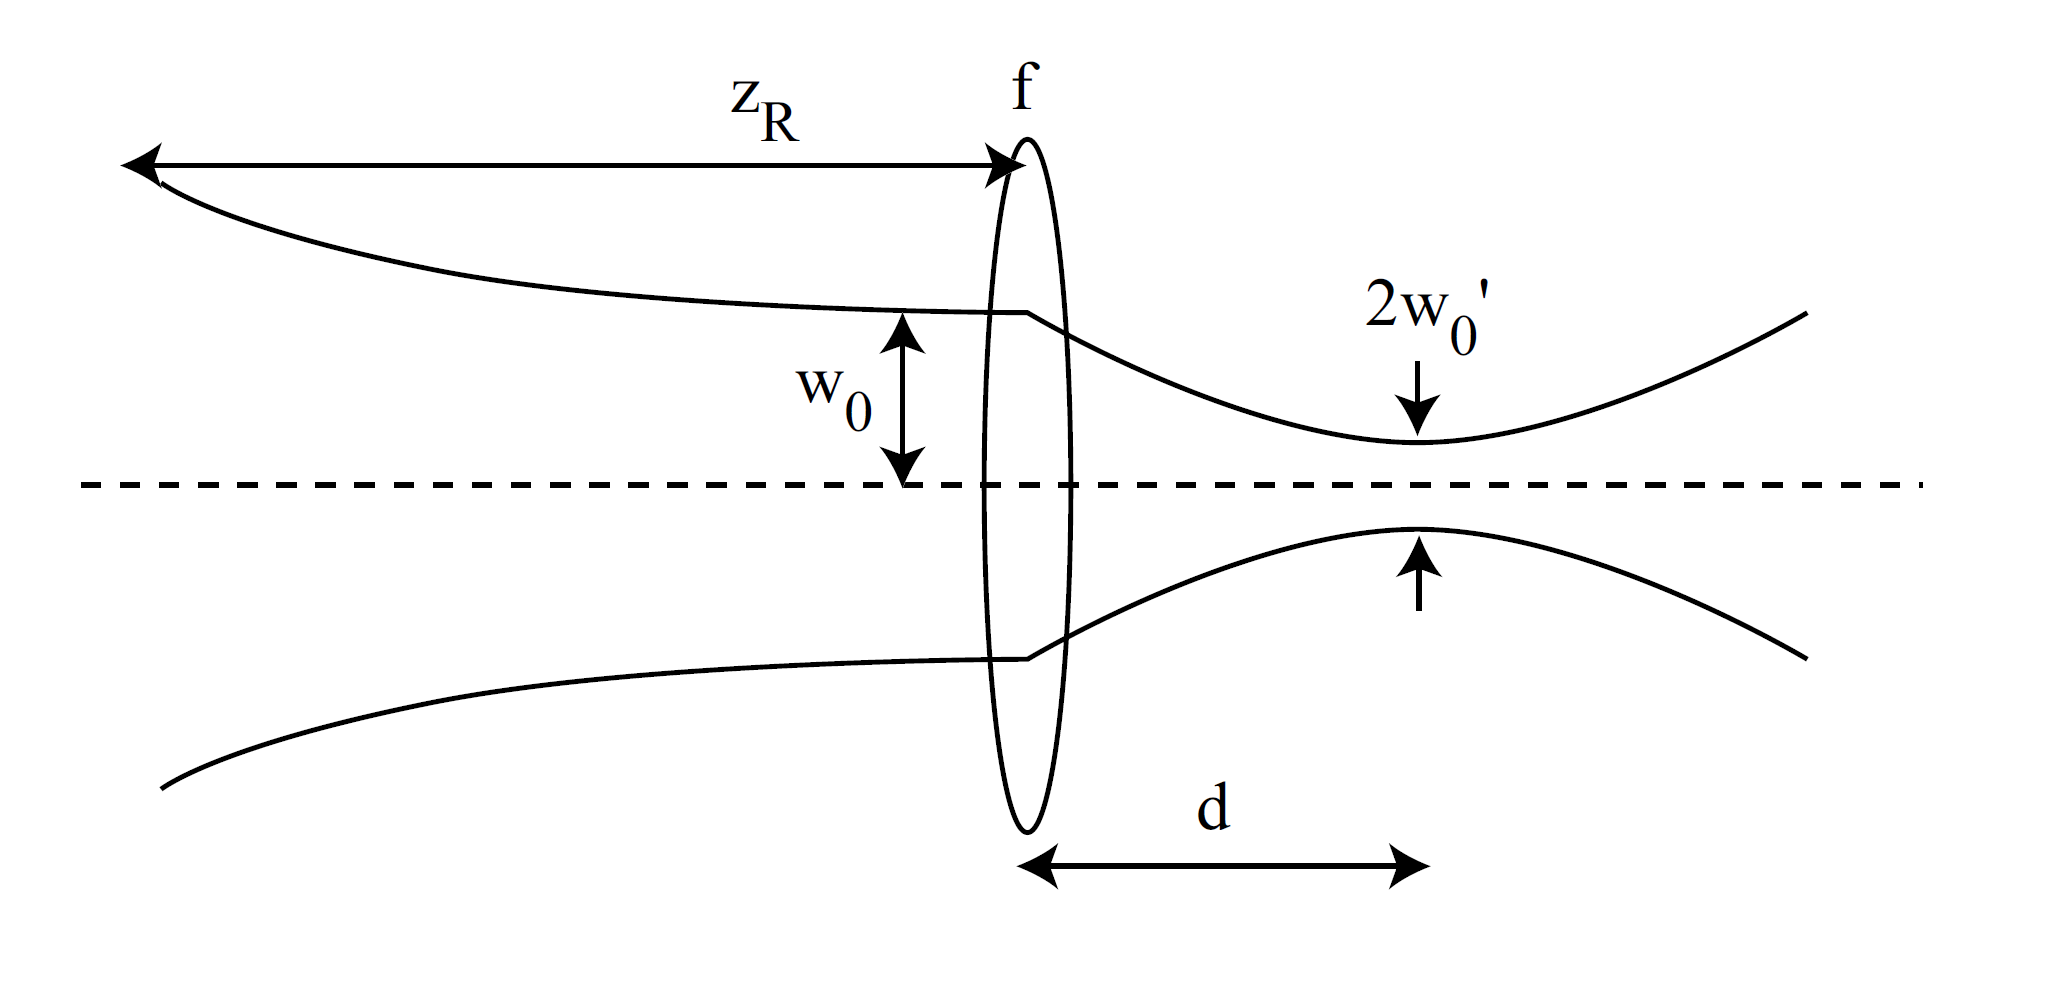
\includegraphics[width=8cm]{question1.png}
	\caption{Representation fo question 1}
	\label{fig2}
\end{figure}

\section{Question 2} % Unnumbered section
By using ABCD matrix, find the q-parameters after passing through the lens with focal length f depending on d. Find the new beam waist  and the distance to it. When $Z_R\ll f$, find the $ \omega_{0}^{'} $ and distance to it in terms of $f$, $\omega_0$ and $\lambda$.


\section*{Slolution}
The ABCD matrix for the thin lens whit focal lenght f is,
\begin{equation}\label{eq10}
\left[
\begin{array}{cc}
1 & 0 \\
-1\//f & 0 \\
\end{array}
\right]
\end{equation}
therefore we could get $q_1$
\begin{equation}\label{eq8}
q_2=\dfrac{q_0}{1-q_1\//f}
\end{equation}
$ q_2 $ follows that,
\begin{equation}\label{eq9}
q_1(z)=z+i\dfrac{n\pi\omega_{0}^{2}}{\lambda}
\end{equation}
The beam  waist locates at the left surface of lens, which means that $z=0, q_1=in\pi\omega_{0}^{2}\//\lambda$. Substitue it into equation \ref{eq2}.

\begin{equation}\label{eq4}
q_2=i\dfrac{fn\pi\omega_{0}^{2}}{\lambda f-in\pi\omega_{0}^{2}}
\end{equation}
We can get the radius and the distance to beam by q parameter.
\begin{equation}\label{eq11}
\begin{array}{l}
\text{Radius of waits:\quad}\omega_{0}^{'}=\sqrt{\dfrac{\lambda}{n\pi}Im\{q{(z)\}}}=\dfrac{\lambda f\omega_{0}}{\sqrt{(\lambda f)^2+(n\pi\omega_0^{2})^2}}

\\
\\
\text{Distance to the waist:\quad} d=-re\{q(z)\}=\dfrac{f(n\pi\omega_0^{2})^2}{(\lambda f)^2+(n\pi\omega_{0}^{2})^2}
\end{array}
\end{equation}
Substitute $ Z_R=n\pi\omega_{0}^{2}\//\lambda $ into equation \ref{eq5}, $\omega_{0}^{'} $ and $ d $ can been written as,
\begin{equation}\label{eq12}
\begin{array}{l}
\omega_{0}^{'}=\dfrac{\omega_0}{\sqrt{1+(Z_R\//f)^2}}
\\
\\
d=\dfrac{f}{1+(f\//Z_R)^2}
\end{array}
\end{equation}
In the case that $ Z_R\gg f $, we ignore the $ f\//Z_R $ term to get that,
\begin{equation}\label{eq13}
\begin{array}{l}
\omega_{0}^{'}=0
\\
\\
d=f
\end{array}
\end{equation}
which indicates that the beam focuses at focus of the lens.
\end{document}



